\documentclass[a0,portrait]{a0poster}
\usepackage[top=3.2cm,bottom=2.5cm,left=3.5cm,right=3.5cm]{geometry}
\usepackage[T1]{fontenc}
\usepackage[utf8]{inputenc}
\usepackage{times}
\usepackage[svgnames]{xcolor}
\usepackage{multicol}
\usepackage{graphicx}
\usepackage{tikz}
\usetikzlibrary{arrows.meta,positioning,fit,shapes.geometric}
\usepackage[most]{tcolorbox}
\usepackage{enumitem}
\usepackage{ragged2e}
\usepackage{microtype}
\usepackage{array}
\usepackage{booktabs}
\pagestyle{empty}

\definecolor{PosterNavy}{HTML}{12355B}
\definecolor{PosterBlue}{HTML}{2176AE}
\definecolor{PosterCyan}{HTML}{2A9D8F}
\definecolor{PosterGold}{HTML}{E9C46A}
\definecolor{PosterRed}{HTML}{C94C4C}
\definecolor{PosterInk}{HTML}{17212B}
\definecolor{PosterLight}{HTML}{F3F7FA}
\definecolor{PosterLine}{HTML}{CBD8E3}

\setlength{\columnsep}{2.0cm}
\setlength{\columnseprule}{0pt}
\setlength{\parindent}{0pt}
\setlength{\parskip}{0.25em}
\setlist[itemize]{leftmargin=1.15em,itemsep=0.16em,topsep=0.18em}

\newtcolorbox{posterbox}[2][]{
  enhanced,
  colback=white,
  colframe=PosterLine,
  boxrule=1.5pt,
  arc=5mm,
  left=7mm,right=7mm,top=4mm,bottom=5mm,
  title={#2},
  coltitle=white,
  colbacktitle=PosterNavy,
  fonttitle=\bfseries\LARGE,
  attach boxed title to top left={xshift=0mm,yshift=-1mm},
  boxed title style={arc=4mm,boxrule=0pt},
  before skip=7mm,after skip=7mm,
  #1
}

\newcommand{\metric}[2]{%
  \begin{minipage}[c]{0.47\linewidth}\centering
  {\color{PosterBlue}\bfseries\LARGE #1}\par
  {\large #2}
  \end{minipage}}

\tikzset{
  stage/.style={rounded corners=3mm,draw=PosterNavy,line width=1.5pt,
    fill=white,minimum height=1.7cm,text width=4.9cm,align=center,
    font=\bfseries\normalsize,inner sep=4mm},
  group/.style={rounded corners=5mm,draw=#1,line width=2pt,fill=none,
    inner sep=6mm},
  flow/.style={-{Latex[length=6mm,width=4mm]},line width=2pt,draw=PosterBlue},
  verify/.style={rounded corners=3mm,draw=PosterCyan,line width=1.5pt,
    fill=PosterCyan!8,minimum height=1.65cm,text width=5.6cm,align=center,
    font=\bfseries\large,inner sep=4mm}
}

\begin{document}
\color{PosterInk}

% Header - preserves the template's title-led identity and navy palette.
\begin{tcolorbox}[
  enhanced,colback=PosterNavy,colframe=PosterNavy,arc=6mm,boxrule=0pt,
  left=15mm,right=15mm,top=11mm,bottom=11mm]
  \begin{minipage}[c]{0.76\linewidth}
    {\color{white}\VeryHuge\bfseries
      Research Paper Assistant using Retrieval-Augmented Generation (RAG)}\\[4mm]
    {\color{PosterGold}\huge
      A Multi-Paper Scientific QA System with Claim-Level Hallucination Verification}
  \end{minipage}\hfill
  \begin{minipage}[c]{0.20\linewidth}
    \centering
    \begin{tikzpicture}
      \node[draw=white,line width=2pt,rounded corners=4mm,
        text=white,align=center,minimum width=10cm,minimum height=5.2cm,
        font=\bfseries\LARGE] {LOCAL\\EVIDENCE-FIRST\\RAG};
    \end{tikzpicture}
  \end{minipage}
\end{tcolorbox}

\vspace{5mm}

% Prominent architecture diagram.
\begin{tcolorbox}[enhanced,colback=PosterLight,colframe=PosterBlue,
  boxrule=2pt,arc=5mm,left=7mm,right=7mm,top=6mm,bottom=6mm]
{\color{PosterNavy}\bfseries\LARGE End-to-end architecture}\par\vspace{4mm}
\centering
\resizebox{0.98\textwidth}{!}{%
\begin{tikzpicture}[node distance=0.7cm]
  \node[stage] (pdf) {PDF Papers};
  \node[stage,right=of pdf] (grobid) {GROBID\\TEI/XML};
  \node[stage,right=of grobid] (sections) {Structured\\Sections};
  \node[stage,right=of sections] (chunks) {Section-Aware\\Chunks};
  \node[stage,right=of chunks] (embed) {Sentence Transformer\\Embeddings};
  \node[stage,right=of embed] (qdrant) {Qdrant\\Vector Index};
  \node[stage,right=of qdrant] (query) {User Query +\\Dense Retrieval};
  \node[stage,right=of query] (rerank) {Cross-Encoder\\Reranking};
  \node[stage,right=of rerank] (llm) {Ollama LLM\\Draft Answer};
  \node[stage,right=of llm] (claims) {Atomic Claim\\Extraction};
  \node[stage,right=of claims] (check) {Claim-Level\\Verification};
  \node[stage,right=of check,fill=PosterCyan!15] (final) {Grounded Answer\\+ Citations};
  \foreach \a/\b in {pdf/grobid,grobid/sections,sections/chunks,chunks/embed,
    embed/qdrant,qdrant/query,query/rerank,rerank/llm,llm/claims,claims/check,check/final}
    \draw[flow] (\a) -- (\b);
  \node[group=PosterBlue,fit=(pdf)(grobid)(sections)(chunks),label={[font=\bfseries\Large,text=PosterBlue]above:Document Processing}] {};
  \node[group=PosterCyan,fit=(embed)(qdrant),label={[font=\bfseries\Large,text=PosterCyan]above:Indexing}] {};
  \node[group=PosterBlue,fit=(query)(rerank),label={[font=\bfseries\Large,text=PosterBlue]above:Retrieval}] {};
  \node[group=PosterCyan,fit=(llm)(claims)(check)(final),label={[font=\bfseries\Large,text=PosterCyan]above:Generation and Verification}] {};
\end{tikzpicture}}
\end{tcolorbox}

\begin{multicols}{3}

\begin{posterbox}{Problem and objective}
Researchers must locate evidence across long, structured papers. General-purpose
language models can answer from outside knowledge or introduce unsupported claims.

\textbf{Objective:} answer single-paper and cross-paper questions using only
retrieved evidence, with citations and claim-level filtering before synthesis.

\begin{itemize}
  \item Ingest multiple scientific PDFs.
  \item Preserve document structure and provenance.
  \item Retrieve and rerank relevant passages.
  \item Compare evidence across named papers.
  \item Remove claims not supported by retrieved excerpts.
\end{itemize}
\end{posterbox}

\begin{posterbox}{Scientific PDF ingestion}
\textbf{GROBID} converts PDFs into structured TEI/XML. The parser retains title,
authors, abstract, sections, subsections, and paragraphs.

\begin{center}

\begin{tikzpicture}[node distance=1.1cm]
  \node[verify] (a) {Scientific PDF};
  \node[verify,right=of a] (b) {GROBID};
  \node[verify,right=of b] (c) {Structured Sections};
  \draw[flow] (a)--(b); \draw[flow] (b)--(c);
\end{tikzpicture}
\end{center}

Structure-aware extraction gives downstream chunks meaningful section context
instead of treating a paper as an undifferentiated text stream.
\end{posterbox}

\begin{posterbox}{Section-aware semantic indexing}
Each chunk retains:
\begin{itemize}
  \item paper title and document name,
  \item section name and chunk ID,
  \item scientific text.
\end{itemize}

\begin{center}
\renewcommand{\arraystretch}{1.3}
\begin{tabular}{>{\bfseries}p{0.38\linewidth}p{0.52\linewidth}}
Embedding model & all-MiniLM-L6-v2 \\
Vector dimension & 384 \\
Vector database & Qdrant \\
Similarity & Cosine similarity \\
\end{tabular}
\end{center}

Dense vectors support semantic search while metadata preserves where every
passage originated.
\end{posterbox}

\begin{posterbox}{Retrieval and reranking}
\begin{center}
\resizebox{0.98\linewidth}{!}{%

\begin{tikzpicture}[node distance=0.75cm]
  \node[verify,text width=4.5cm] (q) {Question};
  \node[verify,right=of q,text width=4.5cm] (e) {Query Embedding};
  \node[verify,right=of e,text width=4.5cm] (d) {Qdrant Candidates};
  \node[verify,right=of d,text width=4.5cm] (r) {Cross-Encoder};
  \node[verify,right=of r,text width=4.5cm] (t) {Top Evidence};
  \foreach \a/\b in {q/e,e/d,d/r,r/t}\draw[flow](\a)--(\b);
\end{tikzpicture}}
\end{center}

Dense retrieval supplies candidates. The
\texttt{ms-marco-MiniLM-L-6-v2} cross-encoder then scores each
question-passage pair and improves evidence ordering.
\end{posterbox}

\columnbreak

\begin{posterbox}[colframe=PosterCyan]{Multi-paper comparison}
Naive global search can over-represent one paper or retrieve a passage that only
mentions the target model. The system resolves the primary subject and routes
atomic claims to the relevant paper before claim-specific retrieval.

\begin{center}
\resizebox{0.98\linewidth}{!}{%
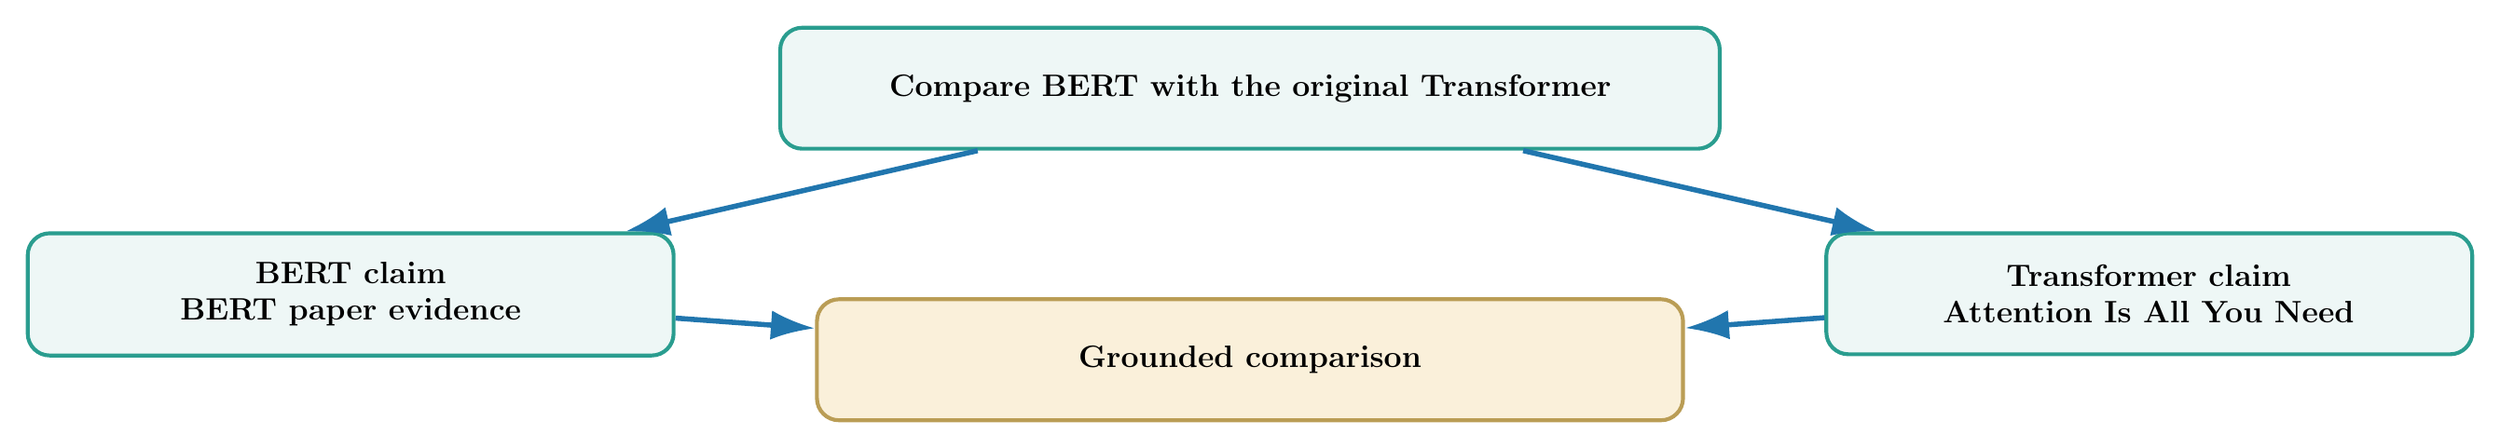
\begin{tikzpicture}[node distance=1.1cm and 1.4cm]
  \node[verify,text width=12cm] (q) {Compare BERT with the original Transformer};
  \node[verify,below left=of q,text width=8cm] (b) {BERT claim\\BERT paper evidence};
  \node[verify,below right=of q,text width=8cm] (t) {Transformer claim\\Attention Is All You Need};
  \node[verify,below=2.0cm of q,text width=11cm,fill=PosterGold!25,draw=PosterGold!80!black] (a) {Grounded comparison};
  \draw[flow] (q)--(b); \draw[flow] (q)--(t);
  \draw[flow] (b)--(a); \draw[flow] (t)--(a);
\end{tikzpicture}}
\end{center}

\textbf{Routing signals:} atomic decomposition, entity detection,
primary-subject identification, referenced-entity distinction, paper filters,
and claim-specific retrieval.
\end{posterbox}

\begin{posterbox}[colframe=PosterCyan]{Claim-level hallucination reduction}
\begin{center}
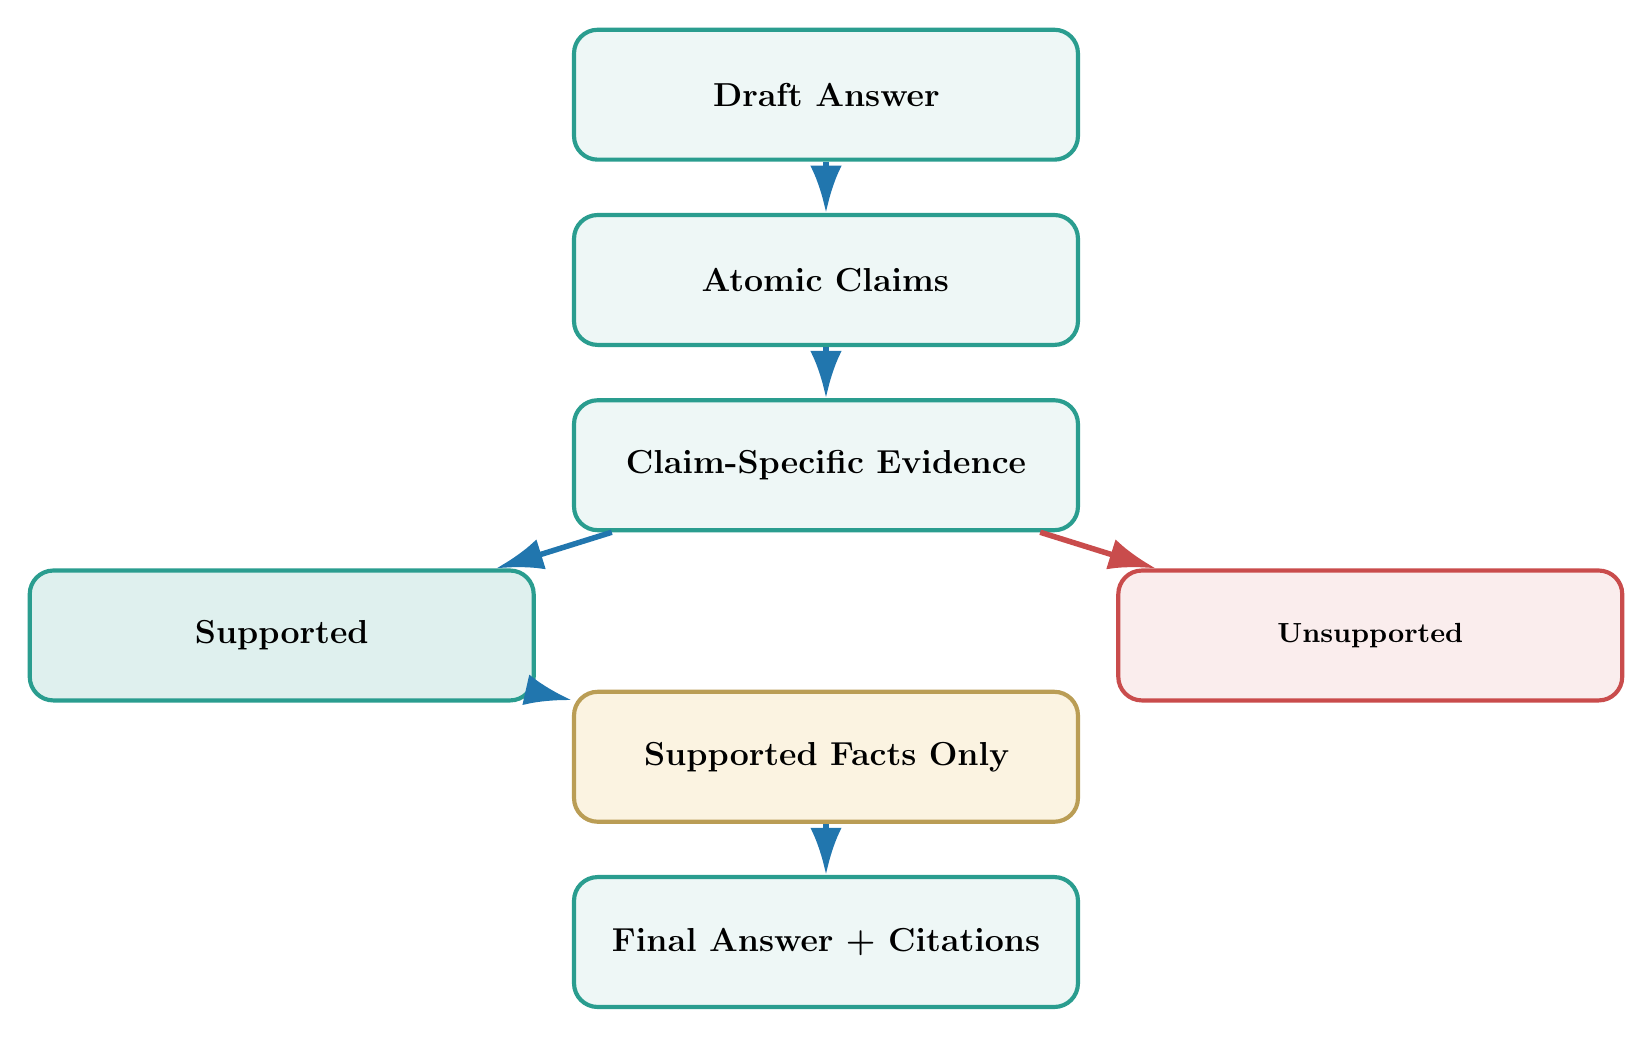
\begin{tikzpicture}[node distance=0.65cm]
  \node[verify] (draft) {Draft Answer};
  \node[verify,below=of draft] (atomic) {Atomic Claims};
  \node[verify,below=of atomic] (ev) {Claim-Specific Evidence};
  \node[verify,below left=of ev,draw=PosterCyan,fill=PosterCyan!15] (yes) {Supported};
  \node[verify,below right=of ev,draw=PosterRed,fill=PosterRed!10,font=\bfseries\normalsize] (no) {Unsupported};
  \node[verify,below=2.0cm of ev,fill=PosterGold!20,draw=PosterGold!80!black] (facts) {Supported Facts Only};
  \node[verify,below=of facts] (answer) {Final Answer + Citations};
  \draw[flow](draft)--(atomic); \draw[flow](atomic)--(ev);
  \draw[flow](ev)--(yes); \draw[flow,draw=PosterRed](ev)--(no);
  \draw[flow](yes)--(facts); \draw[flow](facts)--(answer);
\end{tikzpicture}
\end{center}

The final synthesizer receives verified facts rather than the draft. Source IDs,
paper scope, entity compatibility, duplicates, and malformed partial verdicts
are validated before a fact can reach the answer.
\end{posterbox}

\begin{posterbox}{Verification example}
\textbf{Rejected draft claim}\par
\begin{tcolorbox}[colback=PosterRed!6,colframe=PosterRed,arc=3mm]
``The original Transformer uses constrained self-attention.''
\end{tcolorbox}
The evidence describes masking in the decoder; it does not establish that the
entire architecture uses constrained self-attention. \textbf{Removed.}

\vspace{3mm}
\textbf{Supported claim}\par
\begin{tcolorbox}[colback=PosterCyan!7,colframe=PosterCyan,arc=3mm]
``BERT uses bidirectional self-attention.''
\end{tcolorbox}
Explicitly supported by the BERT model-architecture evidence. \textbf{Retained.}
\end{posterbox}

\begin{posterbox}{Grounded comparison example}
\textbf{Question:} Compare BERT with the original Transformer architecture.

\textbf{BERT}
\begin{itemize}
  \item Multi-layer bidirectional Transformer encoder.
  \item Uses bidirectional self-attention.
  \item Unified architecture across tasks.
\end{itemize}

\textbf{Original Transformer}
\begin{itemize}
  \item Attention-based sequence-transduction model.
  \item Encoder-decoder architecture.
\end{itemize}

\textbf{Key difference:} BERT is encoder-based; the original Transformer has
both encoder and decoder components.

{\small\color{PosterBlue}[Source: BERT, Model Architecture]\quad
[Source: Transformer, Model Architecture]}
\end{posterbox}

\columnbreak

\begin{posterbox}{Evaluation framework implemented}
No completed evaluation run was available in
\texttt{evaluation/results/}; therefore, no performance numbers or charts are
shown.

\textbf{Retrieval evaluation}
\begin{itemize}
  \item Hit@1, Hit@3, Hit@5, and mean reciprocal rank.
  \item Vector retrieval before vs. after reranking.
  \item Paper and section matching.
  \item Comparison-paper coverage.
\end{itemize}

\textbf{Grounding evaluation}
\begin{itemize}
  \item Fully, partially, and unsupported claim rates.
  \item Citation validity and rejected-claim leakage.
  \item Expected-fact coverage and abstention accuracy.
\end{itemize}

\begin{center}
\metric{18}{Evaluation questions}\hfill
\metric{3}{Cross-paper comparisons}\\[5mm]
\metric{2}{Abstention tests}\hfill
\metric{0}{Fabricated metrics}
\end{center}
\end{posterbox}

\begin{posterbox}[colframe=PosterBlue]{Streamlit User Interface}
The Streamlit interface lets users operate the complete RAG pipeline without
notebooks or terminal commands: upload papers, manage the indexed library,
choose a search scope, and ask single-paper or comparison questions.

\begin{center}
\resizebox{0.98\linewidth}{!}{%
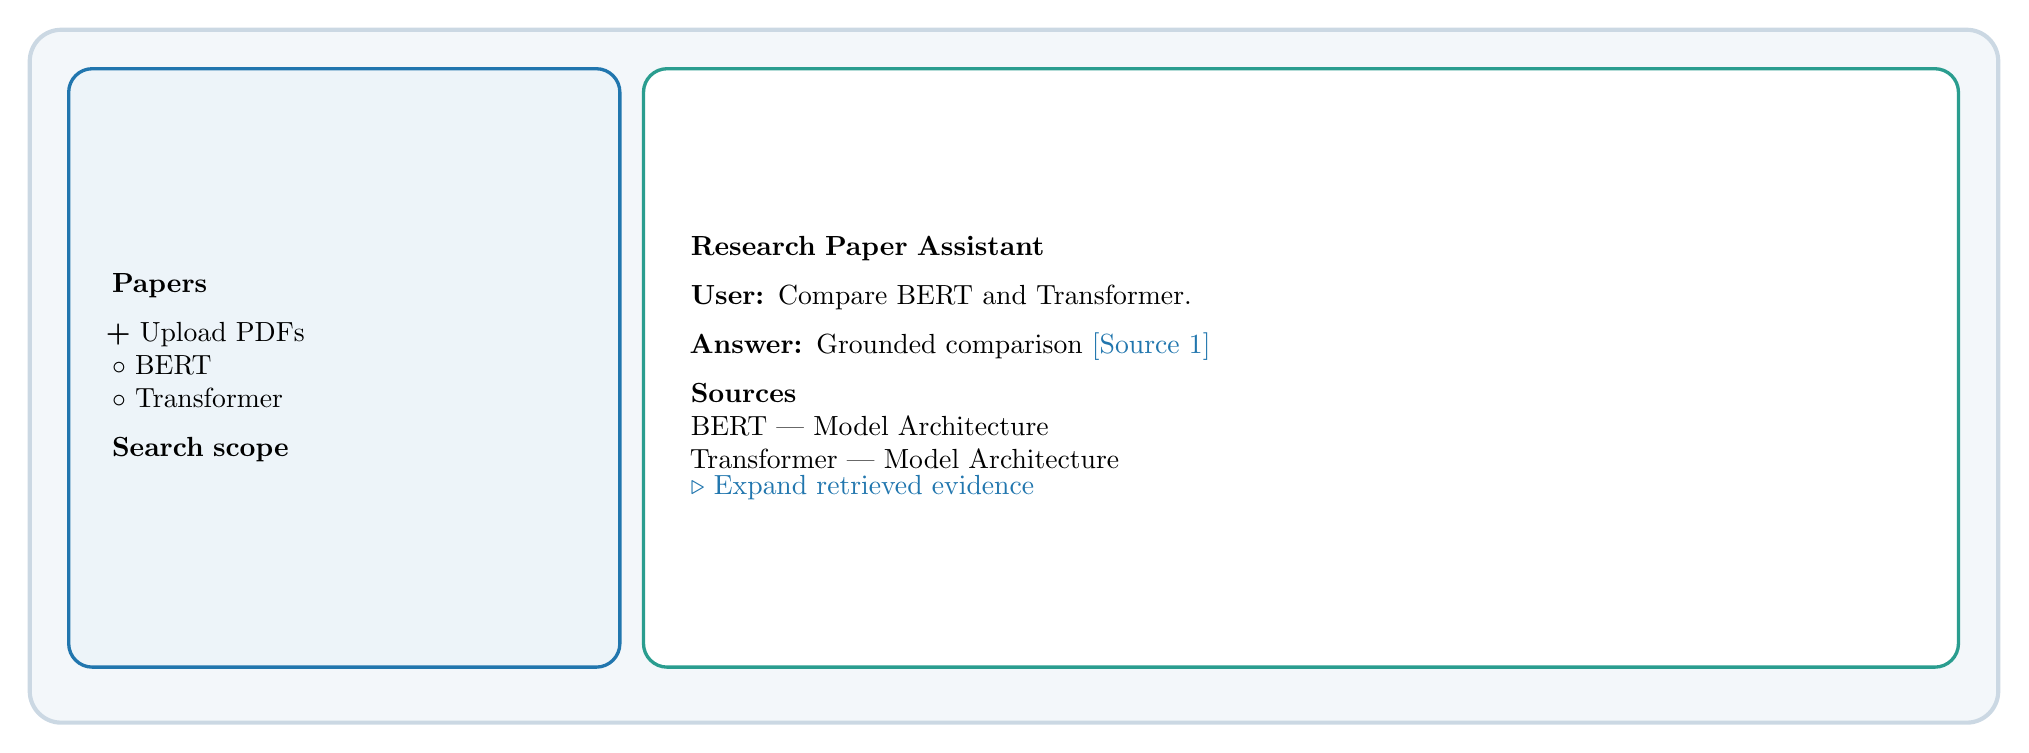
\begin{tikzpicture}[font=\normalsize]
  \node[draw=PosterLine,line width=1.5pt,rounded corners=4mm,
    minimum width=25cm,minimum height=8.8cm,fill=PosterLight] (frame) {};
  \node[anchor=north west,draw=PosterBlue,line width=1.2pt,rounded corners=3mm,
    fill=PosterBlue!8,minimum width=7cm,minimum height=7.6cm,
    text width=5.9cm,align=left,inner sep=5mm]
    at ([xshift=5mm,yshift=-5mm]frame.north west)
    {\textbf{Papers}\\[2mm]
     $\boldsymbol{+}$ Upload PDFs\\
     $\circ$ BERT\\
     $\circ$ Transformer\\[2mm]
     \textbf{Search scope}};
  \node[anchor=north west,draw=PosterCyan,line width=1.2pt,rounded corners=3mm,
    fill=white,minimum width=16.7cm,minimum height=7.6cm,
    text width=15.5cm,align=left,inner sep=5mm]
    at ([xshift=7.8cm,yshift=-5mm]frame.north west)
    {\textbf{Research Paper Assistant}\\[2mm]
     \textbf{User:} Compare BERT and Transformer.\\[2mm]
     \textbf{Answer:} Grounded comparison \textcolor{PosterBlue}{[Source 1]}\\[2mm]
     \textbf{Sources}\\
     BERT --- Model Architecture\\
     Transformer --- Model Architecture\\[-1mm]
     \textcolor{PosterBlue}{$\triangleright$ Expand retrieved evidence}};
\end{tikzpicture}}
\end{center}

\begin{center}
\resizebox{0.96\linewidth}{!}{%

\begin{tikzpicture}[node distance=0.55cm]
  \node[verify,text width=4.0cm] (u) {Upload};
  \node[verify,right=of u,text width=4.0cm] (s) {Select Papers};
  \node[verify,right=of s,text width=4.0cm] (q) {Ask};
  \node[verify,right=of q,text width=4.0cm,font=\bfseries\normalsize] (a) {Grounded Answer};
  \node[verify,right=of a,text width=4.0cm] (e) {View Evidence};
  \foreach \x/\y in {u/s,s/q,q/a,a/e}\draw[flow](\x)--(\y);
\end{tikzpicture}}
\end{center}

\textbf{Transparent answers:} citations expose the paper title, section, and
retrieved chunk behind each answer. Users may expand evidence and optionally
inspect supported and rejected claims.
\end{posterbox}

\begin{posterbox}{Implemented contributions}
\begin{itemize}
  \item Structure-aware scientific PDF ingestion.
  \item Section-aware semantic indexing with provenance.
  \item Dense retrieval plus cross-encoder reranking.
  \item Paper-aware multi-paper evidence routing.
  \item Atomic claim extraction and source-scope verification.
  \item Citation-grounded synthesis and reusable evaluation.
\end{itemize}
\end{posterbox}

\begin{posterbox}{Technology stack}
\begin{center}
\renewcommand{\arraystretch}{1.45}
\begin{tabular}{p{0.30\linewidth}p{0.60\linewidth}}
\textbf{Language} & Python \\
\textbf{Parsing} & GROBID, TEI/XML, PyMuPDF \\
\textbf{Embeddings} & Sentence Transformers \\
\textbf{Vector store} & Qdrant \\
\textbf{Reranking} & Cross-Encoder \\
\textbf{Local LLM} & Ollama, Llama 3.2 3B \\
\textbf{Interface} & Streamlit \\
\textbf{Workflow} & Docker, Jupyter \\
\end{tabular}
\end{center}
\end{posterbox}

\begin{posterbox}{Limitations and future work}
\begin{itemize}
  \item Local LLM verification can make semantic judgment errors.
  \item Dense retrieval can miss highly specific technical evidence.
  \item Claim verification increases inference time.
  \item Next: hybrid retrieval, batched NLI verification, and a larger evaluation set.
\end{itemize}
\end{posterbox}

\begin{posterbox}[colback=PosterNavy,colframe=PosterNavy,coltext=white]{Conclusion}
The system combines structured scientific document processing, semantic
retrieval, reranking, and claim-level verification to produce evidence-grounded
answers across multiple research papers.
\end{posterbox}

\end{multicols}

\vfill
\begin{center}
{\large\color{PosterNavy}\bfseries Research Paper Assistant \textbullet\ Local, source-grounded, multi-paper RAG}
\end{center}

\end{document}
